\input ../SlidePreamble
\input ../preamble


\begin{document}

{\Huge

  \centerline{\bf TTIC 31230, Fundamentals of Deep Learning}
  \bigskip
  \centerline{David McAllester, Autumn 2023}
  \vfill
  \centerline{\bf Generative Adversarial Networks (GANs)}
\vfill
\vfill


\slidetwo{Continuous Cross Entropy is Problematic}{(When the Entropy is Large)}

Suppose we want to train a model of the probability distribution of natural images using cross-entropy loss.

\vfill
$$\Phi^* = \argmin_\Phi \;E_{y \sim \popd}\;-\ln p_\Phi(y)$$

\vfill
Images are continuous stuctured objects --- a continuous value at every pixel.

\vfill
It is difficult to build probability models for sounds or images (or other high-entropy continuous densities)
that both accurately model the distribution and also allow us to calculate $p_\Phi(y)$.

\slide{Generative Adversarial Networks (GANs)}

GANs represent $p_\Phi(y)$ implicitly by constructing an image generator and abandon the ability to compute $p_\Phi(y)$.

\vfill
The cross-entropy loss is replaced by an adversarial discriminator which tries to distinguish between generated images and real images.

\anaslide{Representing a Distribution with a Generator}

\bigskip
\centerline{$z$\hspace{5in}$y_\Phi(z)$}
\centerline{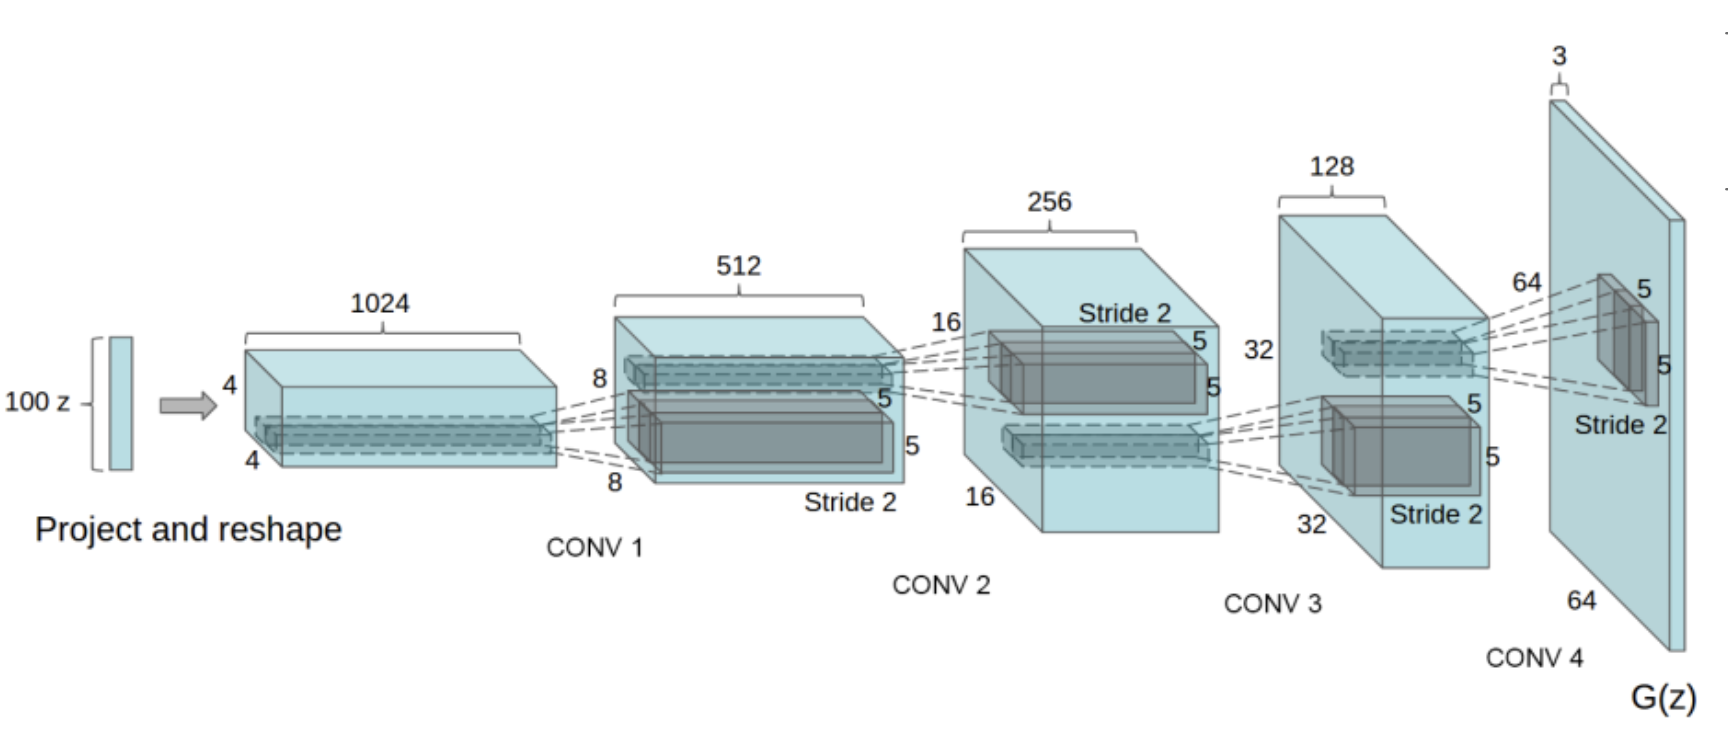
\includegraphics[width=6in]{\images/generator1}}

\bigskip
The random input $z$ defines a probability density on images $y_\Phi(z)$.  We will write this as $p_\Phi(y)$ for the image $y$.

\anaslide{Representing a Distribution with a Generator}

\bigskip
\centerline{$z$\hspace{5in}$y_\Phi(z)$}
\centerline{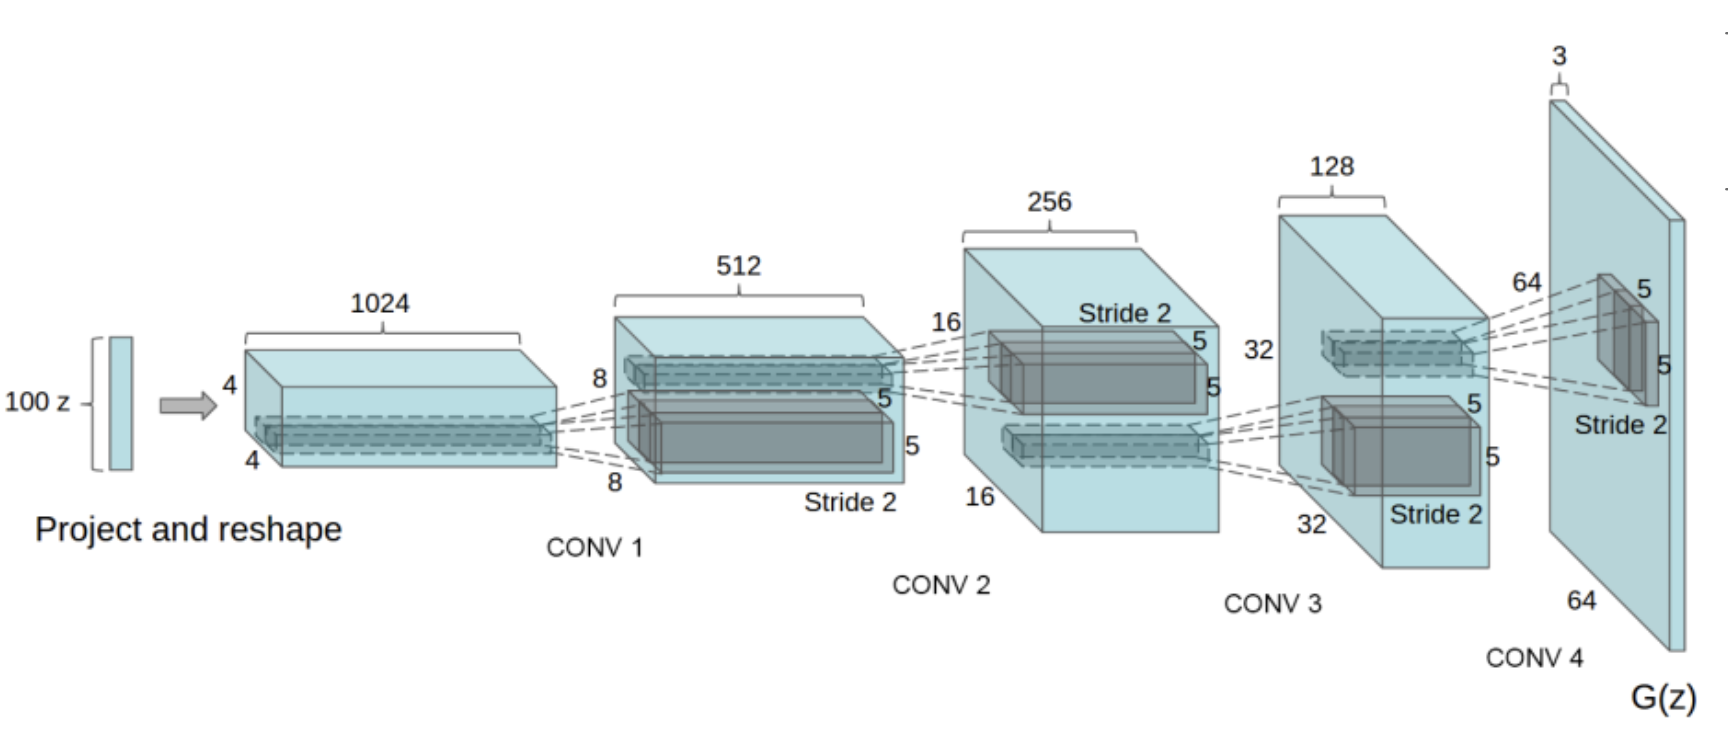
\includegraphics[width=6in]{\images/generator1}}

\bigskip
We want $p_\Phi(y)$ to model a natural image distribution such as the distribution over human faces.


\anaslide{Representing a Distribution with a Generator}

\bigskip
\centerline{$z$\hspace{5in}$y_\Phi(z)$}
\centerline{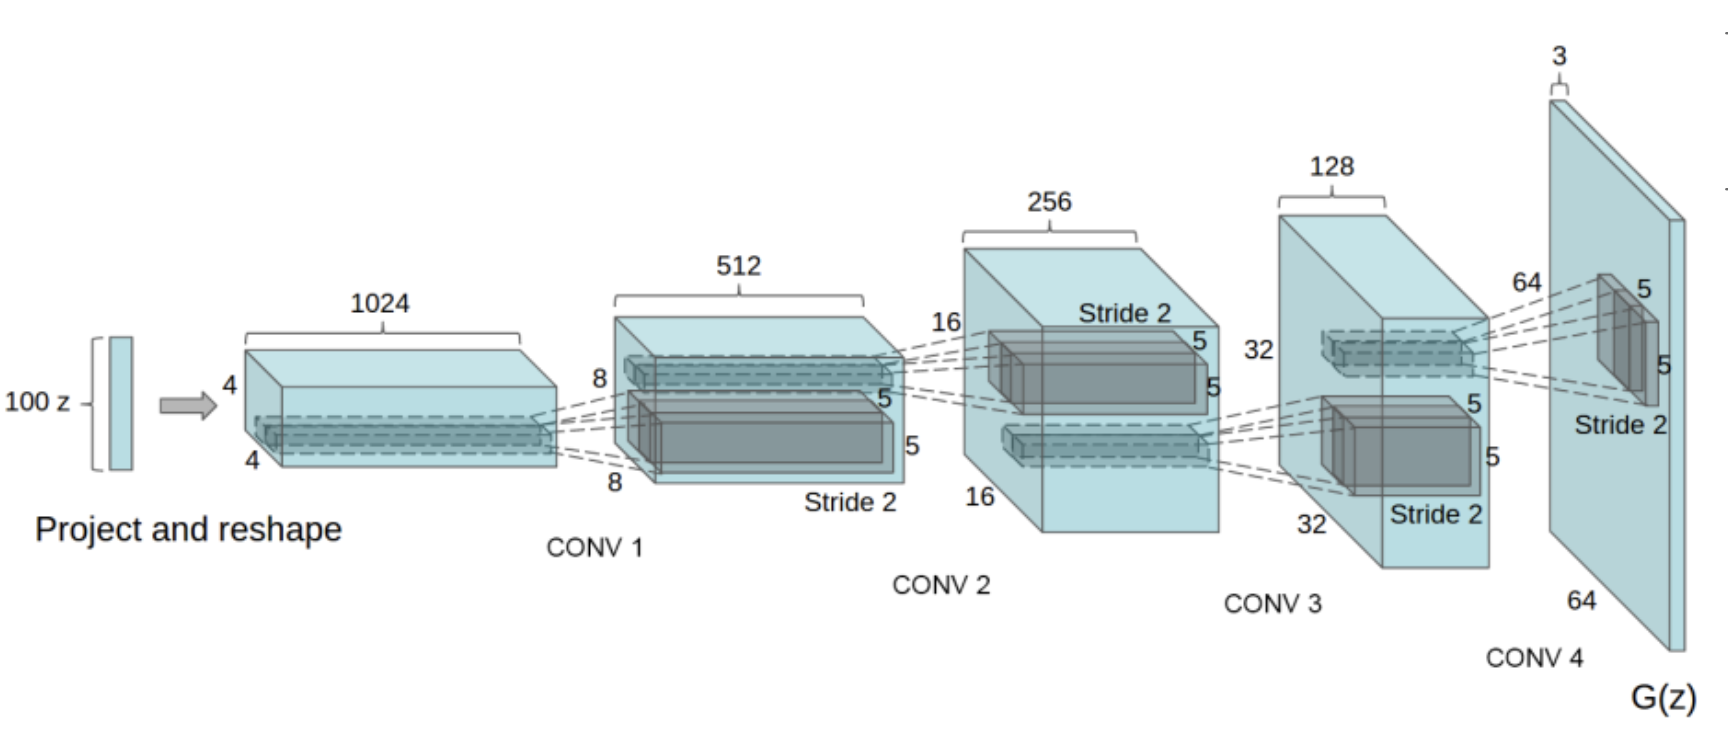
\includegraphics[width=6in]{\images/generator1}}

\bigskip
We can sample from $p_\Phi(y)$ by sampling $z$.  But we cannot compute $p_\Phi(y)$ for $y$ sampled from the population.

\slide{Increasing Spatial Dimension}
 
Reducing spatial dimention with strided convolution:
\begin{tabbing}
For \= $x,y,j,\Delta x,\Delta y, i$ \\
\\
\>$L_{{\ell+1}}[{\color{red}x},{\color{red}y},j]\; \pluseq \;W[\Delta x, \Delta y, i, j] L_{{\ell}}[{\color{red} s*x} + \Delta x, {\color{red} s*y} + \Delta y, i]$
\end{tabbing}

\vfill
Increasing spatial dimension with PyTorch ConvTranspose2d:
\begin{tabbing}
For \= $x,y,j,\Delta x,\Delta y, i$ \\
\\
\>$L_{{\ell+1}}[{\color{red} s*x} + \Delta x, {\color{red} s*y} + \Delta y, i]\; \pluseq \;W[\Delta x, \Delta y, i, j]L_\ell[{\color{red}x},{\color{red}y},j]$
\end{tabbing}

\vfill
{\bf Irrelevant Observation:} ConvTranspose follows the ``swap rule'' for computing gradients for a spacially-reducing Conv layer.

\slide{Generative Adversarial Networks (GANs)}

Let $y$ range over images.  We have a generator $p_\Phi$. For $i \in \{-1,1\}$ we define a probability distribution over pairs
$\tuple{i,y}$ by
\begin{eqnarray*}
\tilde{p}_\Phi(i = 1) & = & 1/2 \\
\tilde{p}_\Phi(y|i=1) & =&  \popd(y) \\
\tilde{p}_\Phi(y|i=-1) & = & p_\Phi(y)
\end{eqnarray*}

\vfill
We also have a discriminator $P_\disc(i|y)$ that tries to determine the source $i$ given the image $y$.

\vfill
The generator tries to fool the discriminator.
\begin{eqnarray*}
        \gen^* & = & \argmax_\gen\;\;\min_\disc\;E_{\tuple{i,y} \sim \tilde{p}_\gen}\;-\ln P_\disc(i|y)
\end{eqnarray*}

\slide{GANs}

The generator tries to fool the discriminator.

\vfill
\begin{eqnarray*}
\gen^* & = & \argmax_\gen\;\;\min_\disc\;E_{\tuple{i,y} \sim \tilde{p}_\gen}\;-\ln P_\disc(i|y)
\end{eqnarray*}

\vfill
{\bf Assuming universality (next slide)} of both the generator $p_\gen$ and the discriminator $P_\disc$ we have {\color{red} $p_{\gen^*} = \popd$}.

\vfill
Note that this involves only discrete cross-entropy.


\slide{The Universality Assumption}

DNNs are universally expressive (can model any function) and trainable (the desired function can be found by SGD).

\vfill
Universality assumption is clearly false but is useful.

\vfill
The success of GANs (to the extent that they have been successful) is a tribute to the utility of the universality ssumption.


\slide{Jensen-Shannon Divergence}

{\huge
\begin{eqnarray*}
  \gen^* & = & \argmax_\gen\;\;\min_\disc\;E_{\tuple{i,y}}\left[-\ln P_\disc(i|y)\right] \\
  \\
  & = & \argmax_\gen E_{\tuple{i,y}}\left[-\ln P(i|y)\right] \\
  \\
    & = & \argmax_\gen \frac{1}{2}E_{y \sim \pop}\left[-\ln P(1|y)\right] + \frac{1}{2} E_{y \sim p_\gen}\left[-P(-1|y)\right] \\
  \\
  & = & \argmin_\gen \; KL\left(\popd,\frac{\popd+p_\gen}{2}\right)+\;KL\left(p_\gen,\frac{\popd+p_\gen}{2}\right) \\
  \\
  \gen^* & = & \argmin_\gen \; {\color{red} \mathrm{JSD}(\popd,p_\gen)}
\end{eqnarray*}
}


\slide{GAN Mode Collapse}

A major concern is ``mode collapse'' where the learned distribution omits a significant fraction of the population distribution.

\vfill
There is no quantitative performance measure that provides a meaningful guarantee against mode collapse.

\vfill
In practice GANS are evaluated on FID score.

\slide{The Fr\'{e}nchet Inception Score (FID)}

Consider two distributions $P$ and $Q$ on $\reals^d$ (perhaps two distributions on images).

\vfill
Generative image models are (still) evaluated using a certain measure of the ``distance'' between the population distribution
and the generation distribution.

\vfill
For GANs we cannot compute the probability of a generated image so we cannot use cross entropy or KL-divergence.

\slide{The Fr\'{e}nchet Inception Score (FID)}

The Fr\'{e}nchet distance $F(P,Q)$ can be measured (approximately) by sampling.

\vfill
Let $\mu$ range over distributions on pairs $(x,y)$ such that

\begin{eqnarray*}
\sum_y \mu(x,y) & = & P(x) \\
\\
\sum_x \mu(x,y) & = & Q(y)
\end{eqnarray*}

$$\mathrm{F}(P,Q) = \inf_{\mu}\;\left(E_{(x,y)\sim \mu} \;||x-y||^2\right)^{\frac{1}{2}}$$

\vfill
This is a form of earth movers distance.  It is also known as the 2-Wasserstein distance.

\slide{The Fr\'{e}nchet Inception Score (FID)}

But rather than measure the $L_2$ distance between images we measure the $L_2$ distance between
the ``inception feature vectors'' $I(x)$ and $I(y)$.

\vfill
For an image $x$ the feature vector $I(x)$ is computed from a certain layer in the inception image classification network.

\slidetwo{Generative Adversarial Nets}{Goodfellow et al., June 2014}
\centerline{\includegraphics[width = 9in]{\images/GAN2014}}
The rightmost column (yellow boarders) gives the nearest neighbor in the training data to the adjacent column.

\slidetwo{Unsupervised Representation Learning ... (DC GANS)}
{Radford et al., Nov. 2015}

\centerline{\includegraphics[width = 9in]{\images/GANDCa}}

\slidetwo{Unsupervised Representation Learning ... (DC GANS)}
{Radford et al., Nov. 2015}

\centerline{\includegraphics[width = 9in]{\images/ImageFeatures}}

\slide{Interpolated Faces}

[Ayan Chakrabarti, January 2017]

\centerline{\includegraphics[height = 4.5in]{\images/interp}}

\slide{Conditional Density Estimation with $L_2$ loss}

Consider training a model $P_\Phi$ to predict the next frame in a video from the two previous frames.

\vfill
$P_\Phi(y_{t+1}|y_t,y_{t+1})$

\vfill
The pair $y_t$ and $y_{t+1}$ give both an image and the motion in the image so predicting
$y_{t+2}$ is possible.

\slide{Conditional Density Estimation with $L_2$ loss}

Here we can train by $L_2$ loss

$$\Phi^* = \argmin_\Phi ||\hat{y}_\Phi(y_t,y_{t-1}) - y_{t+2}||^2$$

\vfill
$L_2$ loss is a special case of cross-entropy loss where $P_\phi(y_{t+2}|y_t,y_{t+1})$ is taken to be a Gaussian centered as
$\hat{y}_\Phi(y_t,y_{t+1})$.


\slide{The General Conditional Case}

We now consider a general conditional case we have a population distribution over pairs $\tuple{x,y}$
where $x$ provides enough information to train the model $\hat{y}_\Phi(y|x)$ by $L_2$ or $L_1$ loss.

\vfill
For the $L_1$ case we have the following.

\vfill
$$\Phi^* = \argmin_\Phi ||\hat{y}_\Phi(y_t,y_{t-1}) - y_{t+2}||_1$$

\slidetwo{Image-to-Image Translation (Pix2Pix)}
{Isola et al., Nov. 2016}

We assume a corpus of ``image translation pairs'' such as images paired with semantic segmentations.

\centerline{\includegraphics[width = 8.0in]{\images/cGAN0}}

\slide{U-Nets}

Pix2Pix uses a U-Net.

\vfill
U-Net: Convolutional Networks for Biomedical Image Segmentation, Ronneberger, Fischer and Brox, May 2015.

\vfill
U-Nets are fundamental to current diffusion models.

\slide{Adversarial Discrimination as an Additional Loss}

$$\gen^* = \argmin_\gen\;E_{(x,y) \sim \popd}\;\; ||y- y_\gen(x)||_1\; {\color{red} + \; \lambda\; {\cal L}_{\mathrm{Discr}}(\gen)}$$

\vfill
$${\cal L}_\mathrm{Discr}(\gen) = \max_\disc \;E_{x,y,i \sim \tilde{p}_\gen}\; \ln P_\disc(i|y,x)$$

\slide{Discrimination as an Additional Loss}

{\huge
$$\begin{array}{lrcl}
\mathrm{L1:} & \gen^* & = & \argmin_\gen\;E_{(x,y) \sim \popd}\;\; ||y - y_\gen(x)||_1 \\
\\
\\
\mathrm{cGAN:} & \gen^* & = & \argmin_\gen\;{\cal L}_{\mathrm{Discr}}(\gen) \\
\\
\\
\mathrm{L1 + cGAN:} & \gen^* & = & \argmin_\gen\;E_{(x,y) \sim \popd}\;\; ||y - y_\gen(x)||_1\; +\; \lambda\; {\cal L}_\mathrm{Discr}(\gen)
\end{array}$$
}


\slidetwo{Image-to-Image Translation (Pix2Pix)}
{Isola et al., Nov. 2016}

\centerline{\includegraphics[height = 4.5in]{\images/cGAN1}}

\slide{Arial Photo to Map and Back}

\centerline{\includegraphics[width = 8.0in]{\images/cGAN2}}

\slidetwo{Unpaired Image-to-Image Translation (Cycle GANs)}{Zhu et al., March 2017}

We have two corpora of images, say images of zebras and unrelated images of horses, or photographs and unrelated paintings by Monet.

\vfill
We want to construct translations between the two classes.

\centerline{\includegraphics[width = 8.0in]{\images/Cycle2}}

\slide{Cycle Gans}

\centerline{\includegraphics[width = 11.0in]{\images/Cycle3}}

\slide{Cycle Gans}

\centerline{\includegraphics[width = 6.0in]{\images/Cycle4}}

\slidetwo{Unsupervised Machine Translation (UMT)}
         {Lample et al, Oct. 2017, also Artetxe et al., Oct. 2017}


In unsupervised machine translation the cycle loss is called {\bf back-translation}.

\slide{Progressive GANs}

\centerline{Progressive Growing of GANs, Karras et al., Oct. 2017}

\centerline{\includegraphics[height = 4.5in]{\images/GANproga}}

\slide{Progressive GANs}

\centerline{\includegraphics[height = 4.5in]{\images/GANprogb}}

\slide{Early GANs on ImageNet}

\centerline{\includegraphics[height = 4.5in]{\images/BadGAN}}

\slide{BigGans}
\centerline{Large Scale GAN Training, Brock et al., Sept. 2018}
\centerline{\includegraphics[width = 9in]{\images/GANclass}}

\vfill
This is a class-conditional GAN --- it is conditioned on the imagenet class label.

\vfill
This generates 512 X 512 images without using progressive training.

\slide{StyleGAN}
{\Large A Style-Based Generator Architecture for Generative Adversarial Networks, Karras et al., Dec. 2018}

\centerline{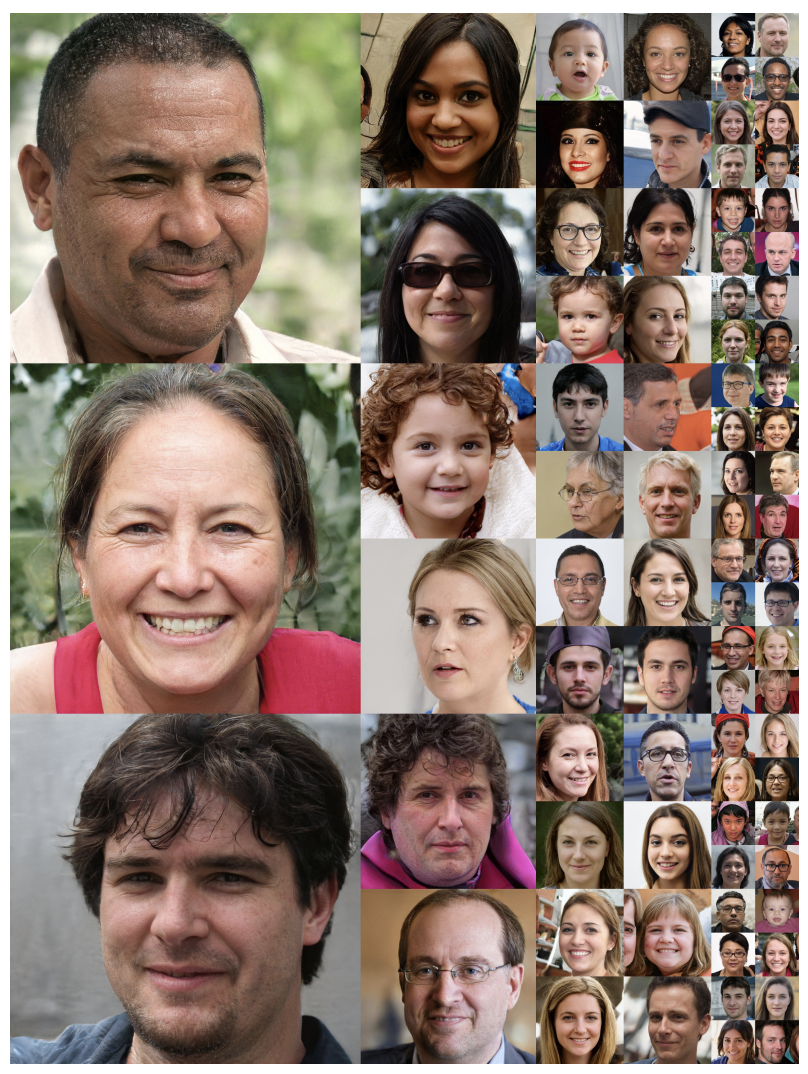
\includegraphics[height= 4.8in]{\images/Style1}}

\slide{StyleGAN: Architecture}

\centerline{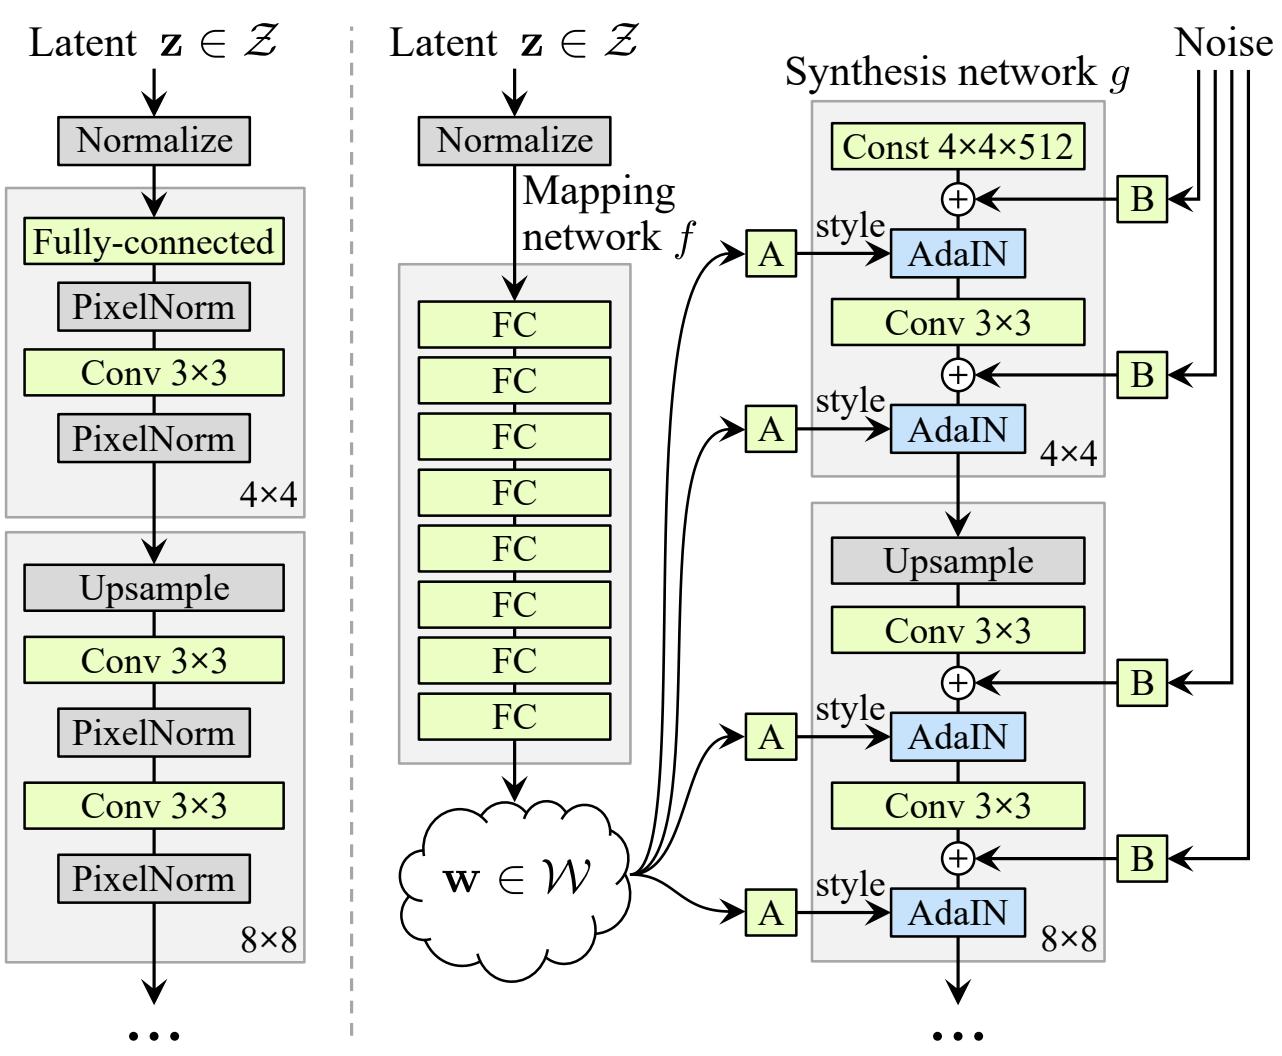
\includegraphics[height= 5.2in]{\images/StyleArch}}

\slide{StyleGAN: Style Transfer}

\centerline{\includegraphics[height= 5.2in]{\images/Style2}}

\slide{StyleGAN: Noise Variation}

\centerline{\includegraphics[height= 5.2in]{\images/Style3}}

\slide{StyleGAN2 and StyleGAN3}

StyleGan2 appeared in December of 2019 with significant improvements.

\vfill
It was demonstrated to work on many classes of images, not just faces.

\vfill
StyleGAN3 appeared in June 2021.

\slide{Projecting Images into Latent Space}

Given an image, can we find a noise vector (a latent vector) that generate a close approximation of
the given image.  Can we invert the generator?

\vfill
We can invert generated images. But we cannot invert (nearly as accurately) newly sampled natural images.

\vfill
By measuring the match between an image $y$ and $g(g^{-1}(y))$ we can determine whether $y$ was generated by StyleGAN2.

\slide{June 2023: StyleGAN Seems to ``Understand'' Images}

\centerline{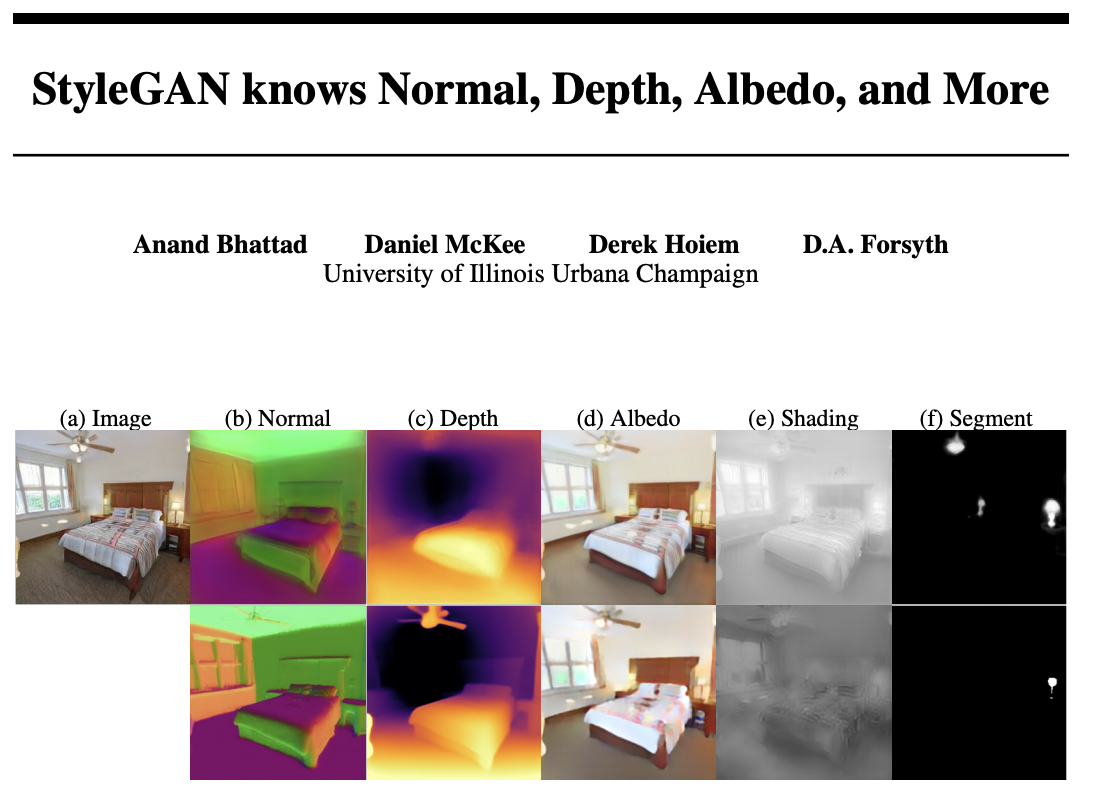
\includegraphics[height= 5.2in]{\images/StyleGANKnows}}

\slide{END}

}
\end{document}

\slide{END}

}
\end{document}
